%------------------------------------------------------------------------------%
\section{Relations}
    \label{Section:ZFC:Elementary_Set_Theory:Relations}%
    \begin{fdefinition}{Relation on a Set}{Relation_on_a_Set}
        A \gls{relation} on a \gls{set} $A$ is a \gls{subset} $R$ of the
        \gls{Cartesian product} $A\times{A}$.
    \end{fdefinition}
    We use a special notation for relations on a set.
    \begin{fnotation}{Relation Notation}{Relation_Notation}
        If $A$ is a set, if $R$ is a relation on $A$, and if $(a,b)\in{R}$, we
        write $aRb$.
        \begin{equation*}
            \forall_{x}\forall_{y}\big(aRb\big)\Leftrightarrow
            \big((a,b)\in{R}\big)
        \end{equation*}
    \end{fnotation}
    For a relation $R$ it is not necessary true that $aRb$ implies $bRa$, nor is
    it necessarily true that $aRa$. These are called symmetric and reflexive
    relations, respectively.
    \begin{lexample}{Examples of Relations}{Examples_of_Relations}
        Let $A=\mathbb{R}$ and consider the relation of equality. That is, let
        $R_{=}\subseteq\mathbb{R}^{2}$ be defined by:
        \begin{equation}
            R_{=}=\{\,(x,y)\in\mathbb{R}^{2}\;|\;x=y\,\}
        \end{equation}
        Then $R_{=}$ is a relation on $\mathbb{R}^{2}$. Rather than writing
        $(x,y)\in{R_{=}}$ or $xR_{=}y$ we commonly write $x=y$. Note that this
        relation is defined entirely by the \textit{diagonal} of the Cartesian
        product $\mathbb{R}\times\mathbb{R}$. Another simple relation is that of
        ordering. Let $R_{<}$ be defined as follows:
        \begin{equation}
            R_{<}=\{\,(x,y)\in\mathbb{R}^{2}\;|\;x<y\,\}
        \end{equation}
        This is also a relation since it is a subset of the Cartesian product,
        but it is a slightly more complicated one. There are many
        \textit{off-diagonal} elements of this relation.
    \end{lexample}
    \begin{theorem}
        If $B$ is a set, if $A\subseteq{B}$, and if $R$ is a relation on $B$,
        then there is a relation $R_{A}$ such that $R_{A}$ is a relation on
        $A$ and $R_{A}\subseteq{R}$.
    \end{theorem}
    \begin{proof}
        For let $P$ be the proposition \textit{True if} $(x,y)\in{A}^{2}$,
        \textit{false otherwise}. By the axiom schema of specification
        (Ax.~\ref{ax:Axiom_Schema_of_Specification}) there is a set:
        \begin{equation}
            R_{A}=\big\{\,(x,y)\in{R}\;|\;P\big((x,y)\big)\,\big\}
        \end{equation}
        But then $(x,y)\in{R}_{A}$ if and only if $(x,y)\in{R}$ and
        $(x,y)\in{A}^{2}$.
    \end{proof}
    This set is called the \textit{restriction} of $R$ to the subset $A$.
    \begin{fdefinition}{Restriction of a Relation}{Restriction_of_a_Relation}
        The restriction of a relation $R$ on a set $B$ to a subset $A$ is the
        set $R_{A}$ defined by:
        \begin{equation*}
            R_{A}=\big\{\,(x,y)\in{R}\;|\;(x,y)\in{A}^{2}\,\big\}
        \end{equation*}
    \end{fdefinition}
    There are many basic properties that relations have, and we prove them now.
    \begin{theorem}
        \label{thm:Cartesian_Product_Is_Relation}%
        If $A$ is a set, then $A\times{A}$ is a relation on $A$.
    \end{theorem}
    \begin{proof}
        For if $A$ is a set, then
        $A\times{A}\subseteq{A}\times{A}$. Therefore, etc.
    \end{proof}
    \begin{theorem}
        \label{thm:Empty_Set_Is_Relation}%
        If $A$ is a set, and then $\emptyset$ is a relation
        on $A$.
    \end{theorem}
    \begin{proof}
        For if $A$ is a set, then
        $\emptyset\subseteq{A}\times{A}$. Therefore, etc.
    \end{proof}
    \begin{theorem}
        Set inclusion $\subseteq$ is a relation. Proper set inclusion
        $\subsetneq$ is a relation. These define partial orderings.
    \end{theorem}
    \begin{fdefinition}{Domain of a Relation}{Domain_of_a_Relation}
        The \gls{domain (relation)} of a \gls{relation} $R$ on a \gls{set} $A$
        is the set:
        \begin{equation*}
            \textrm{dom}(R)=\big\{a\in{A}\;|\;\exists{b}\in{A}
                \textrm{ such that }aRb\big\}
        \end{equation*}
    \end{fdefinition}
    \begin{fdefinition}{Range of a Relation}{Range_of_a_Relation}
        The \gls{range (relation)} of a \gls{relation} $R$ on a \gls{set} $A$ is
        the set:
        \begin{equation*}
            \textrm{ran}(R)=\big\{b\in{A}\;|\;\exists{a}\in{A}
                \textrm{ such that }aRb\big\}
        \end{equation*}
    \end{fdefinition}
    \begin{fdefinition}{Field of a Relation}{Field_of_a_Relation}
        The \gls{field (relation)} of a \gls{relation} $R$ on a set $A$ is the
        set:
        \begin{equation*}
            \textrm{field}(R)=\textrm{dom}(R)\cup\textrm{ran}(R)
        \end{equation*}
        Where $\textrm{dom}(R)$ is the \gls{domain (relation)} of $R$ and
        $\textrm{ran}(R)$ is the \gls{range (relation)} of $R$.
    \end{fdefinition}
    These provide the two most basic examples of relations on a
    set. The empty set is the relation that says no two elements
    are related. Indeed, even single elements are unrelated to
    themselves. The second, the entire Cartesian product
    $A\times{A}$, says that everything is related. These are the
    two extreme cases, but provide useful examples and
    counterexamples in various contexts. More useful is that the
    union and intersection of relations is also a relation. We
    prove this now.
    \begin{theorem}
        \label{thm:Intersection_of_Relations_Is_Relation}%
        If $A$ is a set and if $R_{1}$ and $R_{2}$ are relations
        on $A$, then $R_{1}\cap{R}_{2}$ is a relation on $A$.
    \end{theorem}
    \begin{proof}
        For let $R=R_{1}\cap{R}_{2}$ and suppose $R$ is not a
        relation on $A$. Then there is an $x\in{R}$ such that
        $x\notin{A}\times{A}$. But if $x\in{R}$ then
        $x\in{R}_{1}$ and $x\in{R}_{2}$. But for all
        $x\in{R}_{1}$, $x\in{A}\times{A}$, since $R_{1}$ is a
        relation on $A$, a contradiction as
        $x\notin{A}\times{A}$. Therefore, $R$ is a relation on
        $A$.
    \end{proof}
    \begin{theorem}
        \label{thm:Set_Theory_Union_of_Relations_Is_Relation}
        If $A$ is a set and if $R_{1}$ and $R_{2}$ are relations
        on $A$, then $R_{1}\cup{R}_{2}$ is a relation on $A$.
    \end{theorem}
    \begin{proof}
        For let $R=R_{1}\cup{R}_{2}$ and suppose $R$ is not a
        relation on $A$. Then there is an $x\in{R}$ such that
        $x\notin{A}\times{A}$. But if $x\in{R}$ then
        $x\in{R}_{1}$ or $x\in{R}_{2}$. But for all $x\in{R}_{1}$
        and for all $x\in{R}_{2}$,
        $x\in{A}\times{A}$, since $R_{1}$ and $R_{2}$ are
        relations on $A$, a contradiction. Therefore, etc.
    \end{proof}
    \begin{theorem}
        If $A$ is a set and $R$ is a relation on $A$, then there
        is a relation $\mathcal{U}$ on $A$ such that
        $R\cap\mathcal{U}=R$.
    \end{theorem}
    \begin{proof}
        For let $\mathcal{U}={A}\times{A}$. Then by
        Thm.~\ref{thm:Cartesian_Product_Is_Relation}, $A\times{A}$ is
        a relation on $A$. But since $R$ is a relation,
        $R\subseteq{A}\times{A}$. But then
        $R\cap\mathcal{U}=R$. Therefore, etc.
    \end{proof}
    \begin{theorem}
        If $A$ is a set and $R$ is a relation on $A$, then there
        is a relation $\mathcal{U}$ on $A$ such that
        $R\cup\mathcal{U}=R$
    \end{theorem}
    \begin{proof}
        For let $\mathcal{U}=\emptyset$. Then by
        Thm.~\ref{thm:Empty_Set_Is_Relation},
        $\mathcal{U}$ is a relation. But if $R$ is a set, then
        $R\cup\emptyset=R$. Thus, $R\cup\mathcal{U}=R$.
        Therefore, etc.
    \end{proof}
    Since a general relation is simply a subset of $A\times{A}$,
    there's not much structure on them, and thus there's not a lot
    that can be said about them. We can add more constraints to
    certain relations to get the more familiar properties
    we're used to.
    \begin{fdefinition}{Reflexive Relations}{Reflexive_Relations}
        A reflexive relation on a set $A$ is a
        relation $R$ on $A$ such that for all $a\in{A}$
        it is true that $aRa$.
    \end{fdefinition}
    A reflexive relation on $A$ is simply any subset of
    $A\times{A}$ that contains the entire \textit{diagonal}. That,
    all of the pairs $(a,a)$. A reflexive relation can contain more
    than this, however. The only strict requirement is that
    $aRa$ for all $a\in{A}$.
    \begin{theorem}
        If $A$ is a set, and if $R_{1}$ and $R_{2}$ are reflexive
        relations on $A$, then $R_{1}\cap{R}_{2}$ is a reflexive
        relation on $A$.
    \end{theorem}
    \begin{proof}
        For let $R=R_{1}\cap{R}_{2}$. Then by
        Thm.~\ref{thm:Intersection_of_Relations_Is_Relation}, $R$ is a relation.
        Suppose $R$ is not reflexive.
        Then there is an $a\in{A}$ such that $(a,a)\notin{R}$. But
        if $a\in{A}$, then $(a,a)\in{R}_{1}$, since $R_{1}$ is
        reflexive. Similarly, $(a,a)\in{R}_{2}$ since $R_{2}$ is
        reflexive. But if $(a,a)\in{R}_{1}$ and $(a,a)\in{R}_{2}$,
        then $(a,a)\in{R}$ since $R=R_{1}\cap{R}_{2}$, a
        contradiction. Therefore, $R$ is reflexive.
    \end{proof}
    \begin{theorem}
        If $A$ is a set, if $R_{1}$ is a reflexive relation on
        $A$, and if $R_{2}$ is a relation on $A$, then
        $R_{1}\cup{R}_{2}$ is a reflexive relation on $A$.
    \end{theorem}
    \begin{proof}
        For let $R=R_{1}\cup{R}_{2}$. Since $R_{1}$ and $R_{2}$ are
        relations, by
        Thm.~\ref{thm:Set_Theory_Union_of_Relations_Is_Relation},
        $R$ is a relation. Suppose it is not reflexive.
        Then there is an $a\in{A}$ such that
        $(a,a)\notin{R}$. But if $a\in{A}$ then $(a,a)\in{R}_{1}$
        since $R_{1}$ is reflexive. But if $(a,a)\in{R}_{1}$ then
        $(a,a)\in{R}_{1}\cup{R}_{2}$, a contradiction.
        Therefore, etc.
    \end{proof}
    Given an arbitrary relation $R$ on a set $A$, it may not be
    true that $R$ is reflexive. It may often be useful to add in
    only the necessary points of $A$ that will make $R$
    reflexive. This is called the reflexive closure of $R$.
    \begin{fdefinition}{Reflexive Closure of a Relation}
                       {Reflexive_Closure_of_Relation}
        The reflexive closure of a relation $R$ on a set $A$
        is the set:
        \begin{equation}
            S=R\cup\{(a,a):a\in{A}\}
        \end{equation}
    \end{fdefinition}
    \begin{theorem}
        If $A$ is a set, $R$ is a relation on $A$, and if $S$ is the
        reflexive closure of $R$, then $S$ is a reflexive relation on $A$.
    \end{theorem}
    \begin{theorem}
        \label{thm:Set_Theory_Refl_Clos_Is_Smallest_Refl_With_R}
        If $A$ is a set, if $R$ is a relation on $A$, if
        $S$ is the reflexive closure of $R$, and if $T$ is a
        reflexive relation on $A$ such that $R\subseteq{T}$, then
        $S\subseteq{T}$.
    \end{theorem}
    \begin{proof}
        For if $x\in{S}$, then either $x\in{R}$ or there is an
        $a\in{A}$ such that $x=(a,a)$. But if $x\in{R}$, then
        $x\in{T}$ since $R\subseteq{T}$. If $x\notin{R}$ then
        there is an $a\in{A}$ such that $x=(a,a)$. But $T$ is
        reflexive, and therefore $(a,a)\in{T}$. But then
        $x\in{T}$. Therefore, $S\subseteq{T}$.
    \end{proof}
    Thm.~\ref{thm:Set_Theory_Refl_Clos_Is_Smallest_Refl_With_R}
    says that the reflexive closure of a relation $R$ is, in a sense,
    the \textit{smallest} relation that is reflexive and contains
    $R$ as a subset.
    \begin{theorem}
        If $A$ is a set, $R_{1}$ and $R_{2}$ are relations on $A$,
        and if $S_{1}$ and $S_{2}$ are the reflexive closures of
        $R_{1}$ and $R_{2}$, respectively, then the reflexive closure
        of $R_{1}\cap{R}_{2}$ is:
        \begin{equation}
            S=S_{1}\cap{S}_{2}
        \end{equation}
    \end{theorem}
    \begin{proof}
        By the definition of reflexive closure, we have:
        \begin{align}
            S_{1}&=R_{1}\cup\{(a,a):a\in{A}\}
            \tag{Def.~\ref{def:Reflexive_Closure_of_Relation}}\\
            S_{1}&=R_{2}\cup\{(a,a):a\in{A}\}
            \tag{Def.~\ref{def:Reflexive_Closure_of_Relation}}\\
            \nonumber
            S_{1}\cap{S}_{2}&=
            (R_{1}\cup\{(a,a):a\in{A}\})
            \cap(R_{2}\cup\{(a,a):a\in{A}\})\\
            &=(R_{1}\cap{R}_{2})
            \cup\{(a,a):a\in{A}\}
            \tag{Distributive Law}
        \end{align}
        But by the definition of the transitive closure of
        $R_{1}\cap{R}_{2}$:
        \begin{equation}
            S=(R_{1}\cap{R}_{2})\cup\{(a,a):a\in{A}\}
            \tag{Def.~\ref{def:Reflexive_Closure_of_Relation}}
        \end{equation}
        Therefore, etc.
    \end{proof}
    \begin{fdefinition}{Symmetric Relation}{Symmetric_Relation}
        A symmetric relation on a set $A$ is a
        relation $R$ on $A$ such that for all $a,b\in{A}$
        such that $aRb$, it is true that $bRa$.
    \end{fdefinition}
    \begin{theorem}
        If $A$ is a set, if $S_{1}$ and $S_{2}$ are symmetric relations
        on $A$, then $S_{1}\cap{S}_{2}$ is a symmetric relation on $A$.
    \end{theorem}
    \begin{proof}
        For since $S_{1}$ and $S_{2}$ are relations, $S_{1}\cap{S}_{2}$ is a
        relation (Thm.~\ref{thm:Intersection_of_Relations_Is_Relation}). Suppose
        it is not symmetric. Then there is an $(x,y)\in{S}_{1}\cap{S}_{2}$ such
        that $(y,x)\notin{S}_{1}\cap{S}_{2}$. But if
        $(x,y)\in{S}_{1}\cap{S}_{2}$, then $(x,y)\in{S}_{1}$ and
        $(x,y)\in{S}_{2}$ (Def.~\ref{def:Intersection_of_Two_Sets}). But $S_{1}$
        is symmetric and if $(x,y)\in{S}_{1}$, then $(y,x)\in{S}_{1}$
        (Def.~\ref{def:Symmetric_Relation}). Similarly $(y,x)\in{S}_{2}$, and
        therefore $(y,x)\in{S}_{1}\cap{S}_{2}$
        (Def.~\ref{def:Intersection_of_Two_Sets})), a contradiction. Therefore,
        $S_{1}\cap{S}_{2}$ is symmetric.
    \end{proof}
    \begin{fdefinition}{Transitive Relation}{Transitive_Relation}
        A transitive relation on a set $A$ is a relation $R$ on $A$
        such that for all $a,b,c\in{A}$ such that $aRb$ and $bRc$,
        is it true that $aRc$.
    \end{fdefinition}
    \begin{theorem}
        \label{thm:Entire_Cartesian_is_Transitive}%
        If $A$ is a set, then $A\times{A}$ is a transitive relation on $A$.
    \end{theorem}
    \begin{proof}
        For suppose not. Then there exists $a,b,c\in{A}$ such that
        $(a,b)\in{A}\times{A}$ and $(b,c)\in{A}\times{A}$, yet
        $(a,c)\in{A}\times{A}$. But if $a\in{A}$ and $c\in{A}$, then
        $(a,c)\in{A}\times{A}$ (Def.~\ref{def:Cartesian_Product_of_Two_Sets}), a
        contradiction. Therefore $A\times{A}$ is a transitive relation on $A$.
    \end{proof}
    Using the Cartesian product definition of a relation, we can visualize the
    requirement imposed on transitive relations in the diagram below
    (Fig.~\ref{fig:Transitive_Relation_Diagram}).
    \begin{figure}[H]
        \centering
        \captionsetup{type=figure}
        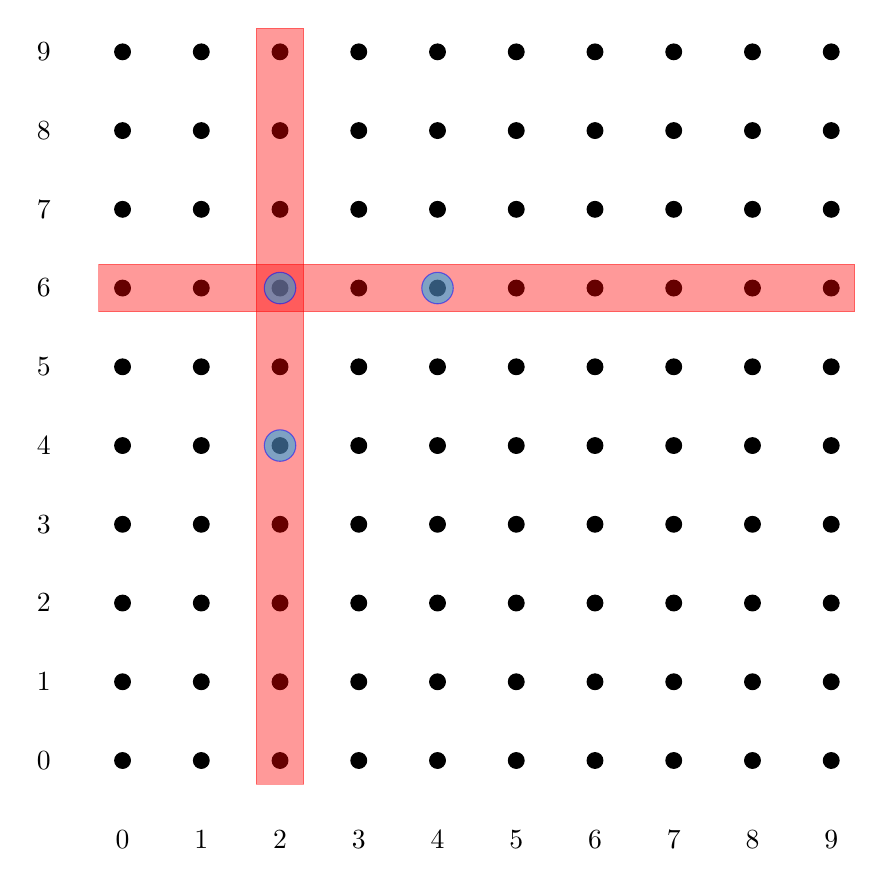
\begin{tikzpicture}
    \foreach\x in {0,1,2,3,4,5,6,7,8,9}{
        \foreach\y in {0,1,2,3,4,5,6,7,8,9}{
            \draw[fill=black] (\x,\y) circle (0.1);
        }
        \node at (\x, -1) {$\x$};
        \node at (-1, \x) {$\x$};
    }

    \draw[fill=red,draw=red,opacity=0.4] ( 1.7, -0.3) rectangle (2.3, 9.3);
    \draw[fill=red,draw=red,opacity=0.4] (-0.3,  5.7) rectangle (9.3, 6.3);

    \draw[draw=blue,fill=cyan,opacity=0.5] (2, 4) circle (0.2);
    \draw[draw=blue,fill=cyan,opacity=0.5] (4, 6) circle (0.2);
    \draw[draw=blue,fill=cyan,opacity=0.5] (2, 6) circle (0.2);
\end{tikzpicture}
        \caption{Diagram for a Transitive Relation}
        \label{fig:Transitive_Relation_Diagram}
    \end{figure}
    Given a point $(a,b)$ that is in the relation and another point $(b,c)$, for
    the relation to be transitive requires $(a,c)$ to be contained in it. That
    is, if we take the first coordinate from the first element and the second
    coordinate from the second element and then combine them to form a new
    ordered pair, this element must also be in the relation.
    \begin{theorem}
        If $A$ is a set, if $T_{1}$ and $T_{2}$ are transitive relations on $A$,
        and if $R=T_{1}\cap{T}_{2}$, then $R$ is a transitive relation.
    \end{theorem}
    \begin{proof}
        For since $T_{1}$ and $T_{2}$ are relations, $T_{1}\cap{T}_{2}$ is a
        relation (Thm.~\ref{thm:Intersection_of_Relations_Is_Relation}). Suppose
        it is not transitive. Then there are $(x,y),(y,z)\in{R}$ such that
        $(x,z)\notin{R}$ (Def.~\ref{def:Transitive_Relation}). But if
        $(x,y),(y,z)\in{R}$, then by the definition of intersection,
        $(x,y),(y,z)\in{T}_{1}$ and $(x,y),(y,z)\in{T}_{1}$
        (Def.~\ref{def:Intersection_of_Two_Sets}). But $T_{1}$ is transitive, and
        thus if $xT_{1}y$ and $yT_{1}z$, then $xT_{1}z$. But similarly $T_{2}$
        is transitive, and therefore $xT_{2}z$. But then $(x,z)\in{T}_{1}$ and
        $(x,z)\in{T}_{2}$, and thus $(x,z)\in{T}_{1}\cap{T}_{2}$, a
        contradiction. Therefore, $R$ is transitive.
    \end{proof}
    \begin{example}
        The requirement that both relations $T_{1}$ and $T_{2}$ are transitive
        cannot be weakened. For consider the relations $S$ and $T$ on
        $\mathbb{Z}_{3}$ defined by:
        \par\hfill\par
        \begin{subequations}
            \begin{minipage}[b]{0.49\textwidth}
                \centering
                \begin{equation}
                    S=\big\{\,(0,1),\,(1,2)\,\}
                \end{equation}
            \end{minipage}
            \hfill
            \begin{minipage}[b]{0.49\textwidth}
                \centering
                \begin{equation}
                    T=\big\{\,(0,1),\,(1,2),\,(0,1)\,\}
                \end{equation}
            \end{minipage}
        \end{subequations}
        \par\vspace{2.5ex}
        Then $T$ is transitive and $S$ is not. Moreover $S\subseteq{T}$, and
        hence $S\cap{T}=S$ (Thm.~\ref{thm:Intersection_with_Subset}), and
        therefore the intersection is not transitive. This example is
        demonstrated in
        Fig.~\subref{fig:Trans_Intersect_Non_Trans_May_Not_Be_Trans}. The
        opposite is possible, and to construct an example we need only find a
        transitve relation $T$ and a non-transitive relation $S$ such that
        $T\subseteq{S}$. Define:
        \par\hfill\par
        \begin{subequations}
            \begin{minipage}[b]{0.49\textwidth}
                \centering
                \begin{equation}
                    T=\big\{\,(0,0)\,\}
                \end{equation}
            \end{minipage}
            \hfill
            \begin{minipage}[b]{0.49\textwidth}
                \centering
                \begin{equation}
                    S=\big\{\,(0,0),\,(0,1),\,(1,2)\,\}
                \end{equation}
            \end{minipage}
        \end{subequations}
        \par\vspace{2.5ex}
        Then $T$ is transitive, $S$ is not, and $S\cap{T}=T$
        (See \subref{fig:Trans_Int_Trans_May_Not_Be_Trans}).
    \end{example}
    \begin{figure}[H]
        \centering
        \captionsetup{type=figure}
        \begin{subfigure}[b]{0.49\textwidth}
            \centering
            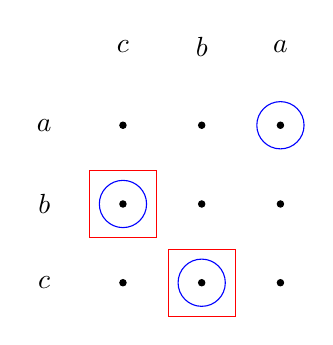
\begin{tikzpicture}
    \foreach\x in {0,1,2}{
        \foreach\y in {0,1,2}{
            \draw[fill=black] (\x,\y) circle (0.4mm);
        }
    }
    \node at (-1, 2) {$a$};
    \node at (-1, 1) {$b$};
    \node at (-1, 0) {$c$};
    \node at (2, 3) {$a$};
    \node at (1, 3) {$b$};
    \node at (0, 3) {$c$};
    \draw[draw=blue,fill=none] (0,1) circle (0.3);
    \draw[draw=blue,fill=none] (1,0) circle (0.3);
    \draw[draw=blue,fill=none] (2,2) circle (0.3);
    \draw[draw=red,fill=none] (-0.4243, 0.5757) rectangle (0.4243, 1.4243);
    \draw[draw=red,fill=none] ( 0.5757,-0.4243) rectangle (1.4243, 0.4243);
\end{tikzpicture}
            \subcaption{The intersection is not transitive}
            \label{fig:Trans_Intersect_Non_Trans_May_Not_Be_Trans}
        \end{subfigure}
        \hfill
        \begin{subfigure}[b]{0.49\textwidth}
            \centering
            \begin{tikzpicture}
    \foreach\x in {0,1,2}{
        \foreach\y in {0,1,2}{
            \draw[fill=black] (\x,\y) circle (0.4mm);
        }
    }
    \node at (-1, 2) {$a$};
    \node at (-1, 1) {$b$};
    \node at (-1, 0) {$c$};
    \node at (2, 3) {$a$};
    \node at (1, 3) {$b$};
    \node at (0, 3) {$c$};
    \draw[draw=blue,fill=none] (0,2) circle (0.3);
    \draw[draw=red,fill=none] (-0.4243, 1.5557) rectangle (0.4243, 2.4243);
    \draw[draw=red,fill=none] (-0.4243, 0.5757) rectangle (0.4243, 1.4243);
    \draw[draw=red,fill=none] ( 0.5757,-0.4243) rectangle (1.4243, 0.4243);
\end{tikzpicture}
            \subcaption{The intersection is transitive}
            \label{fig:Trans_Int_Trans_May_Not_Be_Trans}
        \end{subfigure}
        \label{fig:Intersection_of_Transitive_and_Non_Transitive_Relations}
        \caption{The Intersection of Transitive and Non-Transitive Relations}
    \end{figure}
    We can strengthened our claim that the intersection of two transitive
    relations is again transitive and show that any arbitrary intersection will
    again be transitive.
    \begin{theorem}
        \label{thm:Intersection_of_Transitive_is_Transitive}%
        If $A$ is a set, if $\mathcal{P}(A\times{A})$ denotes the power set of
        $A\times{A}$, if $\mathcal{O}\subseteq\mathcal{P}(A\times{A})$ is such
        that for all $\mathcal{U}\in\mathcal{O}$ it is true that $\mathcal{U}$
        is a transitive relation on $A$, if $\mathcal{T}$ is defined by:
        \begin{equation}
            \mathcal{T}=\bigcap_{\mathcal{U}\in\mathcal{O}}\mathcal{U}
        \end{equation}
        Then $\mathcal{T}$ is a transitive relation on $A$.
    \end{theorem}
    \begin{proof}
        For suppose not. Then there exists $a,b,c\in{A}$ such that
        $(a,b)\in\mathcal{T}$ and $(b,c)\in\mathcal{T}$, yet
        $(a,c)\notin\mathcal{T}$. But if $(a,b)\in\mathcal{T}$, then for all
        $\mathcal{U}\in\mathcal{O}$ it is true that $(a,b)\in\mathcal{U}$
        (Def.~\ref{def:Intersection_Over_a_Collection}). Similarly, for all
        $\mathcal{U}\in\mathcal{O}$ it is true that $(b,c)\in\mathcal{U}$.
        But by hypothesis, for all $\mathcal{U}\in\mathcal{O}$ it is true that
        $\mathcal{U}$ is a transitive relation and thus if $(a,b)\in\mathcal{U}$
        and $(b,c)\in\mathcal{U}$, then it is true that $(a,c)\in\mathcal{U}$
        (Def.~\ref{def:Transitive_Relation}). But then for all
        $\mathcal{U}\in\mathcal{O}$ it is true that $(a,c)\in\mathcal{U}$, and
        therefore $(a,c)\in\mathcal{T}$
        (Def.~\ref{def:Intersection_Over_a_Collection}), a contradiction.
        Therefore, $\mathcal{T}$ is a transitive relation on $A$.
    \end{proof}
    This allows us to define the transitive closure of any relation $R$ on a set
    $A$. It is, in a sense, the \textit{smallest} transitive relation that
    contains $R$.
    \begin{theorem}
        If $A$ is a set and if $R$ is a relation on $A$, then there exists a
        transitive relation $\mathcal{T}$ on $A$ such that
        $R\subseteq\mathcal{T}$ and such that for transitive relations $T$ on
        $A$ such that $R\subseteq{T}$ it is true that $\mathcal{T}\subseteq{T}$.
    \end{theorem}
    \begin{proof}
        For let $P$ be the proposition \textit{True if} $S$
        \textit{is a transitive relation on} $A$ \textit{such that}
        $R\subseteq{S}$, \textit{false otherwise}. Then by the axiom schema of
        specification (Ax.~\ref{ax:Axiom_Schema_of_Specification}) there exists
        a set:
        \begin{equation}
            \mathcal{O}=\big\{\,S\in\mathcal{P}(A\times{A})\;|\;P(S)\,\big\}
        \end{equation}
        But then for all $S\in\mathcal{O}$, $P(S)$ is true and therefore
        $R\subseteq{S}$ and $S$ is transitive. Moreover, $\mathcal{O}$ is
        non-empty since by Thm.~\ref{thm:Entire_Cartesian_is_Transitive},
        $A\times{A}$ is a transitive relation. Define $\mathcal{T}$ by:
        \begin{equation}
            \mathcal{T}=\bigcap_{S\in\mathcal{O}}S
        \end{equation}
        Then by Thm.~\ref{thm:Intersection_of_Transitive_is_Transitive},
        $\mathcal{T}$ is a transitive relation. Moreover, suppose $S$ is a
        transitive relation such that $R\subseteq{S}$. But if $S$ is a relation
        on $A$, then $S\subseteq{A}\times{A}$
        (Def.~\ref{def:Relation_on_a_Set}) and therefore
        $S\in\mathcal{P}(A\times{A})$ (Def.~\ref{def:Power_Set}). But if $S$ is
        a transitive relation and if $R\subseteq{S}$, then $P(S)$ is true, and
        therefore $S\in\mathcal{P}$. Thus, $\mathcal{T}\subseteq{S}$.
    \end{proof}
    \begin{fdefinition}{Transitive Closure}{Transitive_Closure}
        The transitive closure of a relation $R$ on a set
        $A$ is the the set $R^{t}\subseteq{A}\times{A}$ defined by:
        \begin{equation}
            R^{t}
        \end{equation}
    \end{fdefinition}
    \begin{fdefinition}{Asymmetric Relation}{Assymetric_Relation}
        An asymmetric relation on a set $A$ is a relation $R$
        on $A$ such that for all $a,b\in{A}$ such that $aRb$
        it is true that $(b,a)\notin{R}$.
    \end{fdefinition}
    \begin{fdefinition}{Total Relation}{Total_Relation}
        A total relation on a set $A$ is a relation $R$ on $A$ such
        that for all $a,b\in{A}$ it is true that either
        $aRb$ or $bRa$, or both.
    \end{fdefinition}
    The notion of equality can be defined as a relation
    with the following properties:
    \begin{enumerate}
        \item Equality is Reflexive: $a=a$ for all $a\in{A}$.
        \item Equality is Symmetric: $a=b$ if and only if $b=a$.
        \item Equality is Transitive: If $a=b$ and $b=c$, then $a=c$.
        \item The relation is uniquely defined by the set
              $\{(a,a)\in A\times A:a\in A\}$.
    \end{enumerate}
    That is, equality can be seen as the \textit{diagonal} in the
    Cartesian product $A\times{A}$.
    \begin{fdefinition}{Antisymmetric Relation}
        An antisymmetric relation on a set $A$ is a relation $R$ on $A$
        such that for all $a,b\in{A}$ such that $aRb$ and $bRa$, it
        is true that $a=b$.
    \end{fdefinition}
    \begin{fdefinition}{Equivalence Relation}{Equivalence_Relation}
        An equivalence relation on a set $A$ is a relation $R$ on $A$ such that
        $R$ is reflexive, symmetric, and transitive.
    \end{fdefinition}
    Equivalence relations attempt to model equality. They are fundamental in
    mathematics as they allow us to define \textit{equivalence classes}, which
    are used to define quotients. There are many examples such as quotient
    topologies, quotient groups, quotient rings, and quotient modules, all of
    which will be discussed later.
    \begin{fdefinition}{Equivalence Class}{Equivalence_Class}
        The equivalence class of an element $x$ in a set $A$ by an
        equivalence relation $R$ is the set:
        \begin{equation*}
            [x]=\{\,y\in{A}\;|\;xRy\,\}
        \end{equation*}
    \end{fdefinition}
    It's important to note that the term class here is different from the notion
    of a collection of sets. And equivalence class of an element $x$ in a set
    $A$ under an equivalene relation $R$ will indeed be a set in $ZFC$.
    \begin{theorem}
        \label{thm:Equivalence_Classes_Disjoint_or_Equal}%
        If $A$ is a set, if $R$ is an equivalence relation on $A$, and if
        $x,y\in{A}$, then either $[x]=[y]$ or $[x]\cap[y]=\emptyset$.
    \end{theorem}
    \begin{proof}
        For suppose not and suppose $[x]\ne[y]$ and that
        $[x]\cap[y]\ne\emptyset$. That is, suppose:
        \begin{equation*}
            \neg([x]=[y])\land\neg([x]\cap[y]=\emptyset)
        \end{equation*}
        If $[x]\cap[y]$ is non-empty then there is a
        $z\in{A}$ such that $z\in[x]$ and $z\in[y]$
        (Def.~\ref{def:Non_Empty_Set}). But if $z\in[x]$, then $xRz$
        (Def.~\ref{def:Equivalence_Class}). But also
        $z\in[y]$ and therefore $yRz$. But $R$ is an equivalence relation and
        is therefore symmetric (Def.~\ref{def:Equivalence_Relation}) and thus
        if $yRz$ then $zRy$ (Def.~\ref{def:Symmetric_Relation}). But an
        equivalence relation is also transitive, and thus if $xRz$ and $zRy$,
        then $xRy$ (Def.~\ref{def:Transitive_Relation}). But if $[x]\ne[y]$ then
        either $[x]\nsubseteq[y]$ or $[y]\nsubseteq[x]$. Suppose
        $[x]\nsubseteq[y]$ and let $a\in[x]$ be such that $a\notin[y]$. But
        if $a\in[x]$ then $xRa$ (Def.~\ref{def:Equivalence_Class}). But since
        equivalence relations are symmetric, if $xRa$, then $aRx$. But it was
        proven that $xRy$ and since equivalence relations are transitive, if
        $aRx$ and $xRy$, then $aRy$. But again if $aRy$, then $yRa$ and
        therefore $a\in[y]$, a contradiction. Therefore $[x]\subseteq[y]$.
        Similarly, $[y]\subseteq[x]$ and therefore $[x]=[y]$, a contradiction.
        By the law of the excluded middle, the negation is true:
        \begin{equation*}
            \neg\big(\neg([x]=[y])\land\neg([x]\cap[y]=\emptyset)\big)
            =([x]=[y])\lor([x]\cap[y]=\emptyset)
        \end{equation*}
        Thus, either $[x]=[y]$ or $[x]\cap[y]=\emptyset$.
    \end{proof}
    \begin{fdefinition}{Quotient Set}{Quotient_Set}
        The quotient set of a set $A$ by an equivalence relation $R$ on $A$ is
        the set:
        \begin{equation*}
            A/R=\{\,[x]\in\mathcal{P}(A)\;|\;x\in{A}\,\}
        \end{equation*}
        Where $[x]$ is the equivalence class of $x$ under $R$.
    \end{fdefinition}
    \begin{example}
        The definition of the quotient set comes naturally when one considers
        functions between sets. Suppose $A$ and $B$ are sets, and suppose
        $f:A\rightarrow{B}$ is a function. In general, it may not be true that
        $f(a_{1})=f(a_{2})$ implies that $a_{1}=a_{2}$, and so we wish to find a
        subset of $A$ with this property. The quotient set does this. Let
        $R$ be the relation:
        \begin{equation}
            R=\{\,(a,b)\in{A}^{2}\;|\;f(a)=f(b)\,\}
        \end{equation}
        If we form the quotient set $A/R$ and consider the projective mapping
        $\pi:A\rightarrow{A}/R$ that sends $a\in{A}$ to its equivalence class.
        That is, $\pi(a)=[a]$. We then seek a function
        $\tilde{f}:A/R\rightarrow{B}$ such that $\tilde{f}\circ{\pi}=f$.
        That is, we wish to make the diagram below \textit{commute}.
        \begin{figure}[H]
            \centering
            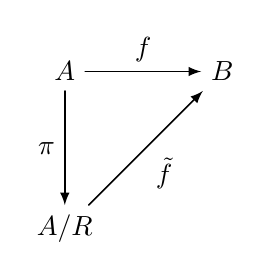
\begin{tikzpicture}[%
    >=latex,
    every path/.style={->},
    line width=0.2mm,
    line cap=round
]
    \node (A) at (0.0,  0.0) {$A$};
    \node (AR) at (0.0, -2.0) {$A/R$};
    \node (B) at  (2.0,  0.0) {$B$};
    \path (A) edge node [above]        {$f$}         (B);
    \path (AR) edge node [below right] {$\tilde{f}$} (B);
    \path (A) edge node [left]         {$\pi$}       (AR);
\end{tikzpicture}
            \label{fig:Comm_Diagram_Quotient_Set}
            \caption{Commutative Diagram for the Quotient Set}
        \end{figure}
        So we need to map $[x]$ to $f(x)$. That is, $\tilde{f}([x])=f(x)$. For
        this problem to be well posed requires that the equivalence class that
        make up the elements of $A/R$ come from equivalence relations. That is,
        that the relation $R$ is transitive, symmetric, and reflexive.
    \end{example}
    \begin{theorem}
        If $A$ is a set and if $R$ is an equivalence relation on $A$, then
        $A/R$ is a partition of $A$.
    \end{theorem}
    \begin{proof}
        For by Thm.~\ref{thm:Equivalence_Classes_Disjoint_or_Equal}, if
        $\mathcal{U},\mathcal{V}\in{A}/R$, then either
        $\mathcal{U}=\mathcal{V}$ or $\mathcal{U}\cap\mathcal{V}=\emptyset$.
        But also, for all $x\in{A}$, there is a $\mathcal{U}\in{A}/R$ such that
        $x\in\mathcal{U}$ since $x\in[x]$ and $[x]\in{R}/A$. Therefore,
        $A/R$ is a partition of $A$.
    \end{proof}